\indent

This section presents an \textbf{overview of the entire system requirements} through a high-level use case diagram. It also includes details visualizations of each \textbf{key module and feature under my responsibility}.


\subsubsection{System Requirements Overview}
\noindent
\begin{minipage}{\textwidth}
    \setlength{\parindent}{2em}
    From the modules and user roles defined in \textbf{\autoref{sec:scope} \nameref{sec:scope}}, this section presents a visual overview of the entire systems requirements and the associated user roles.
\end{minipage}

\begin{figure}[H]
    \centering
    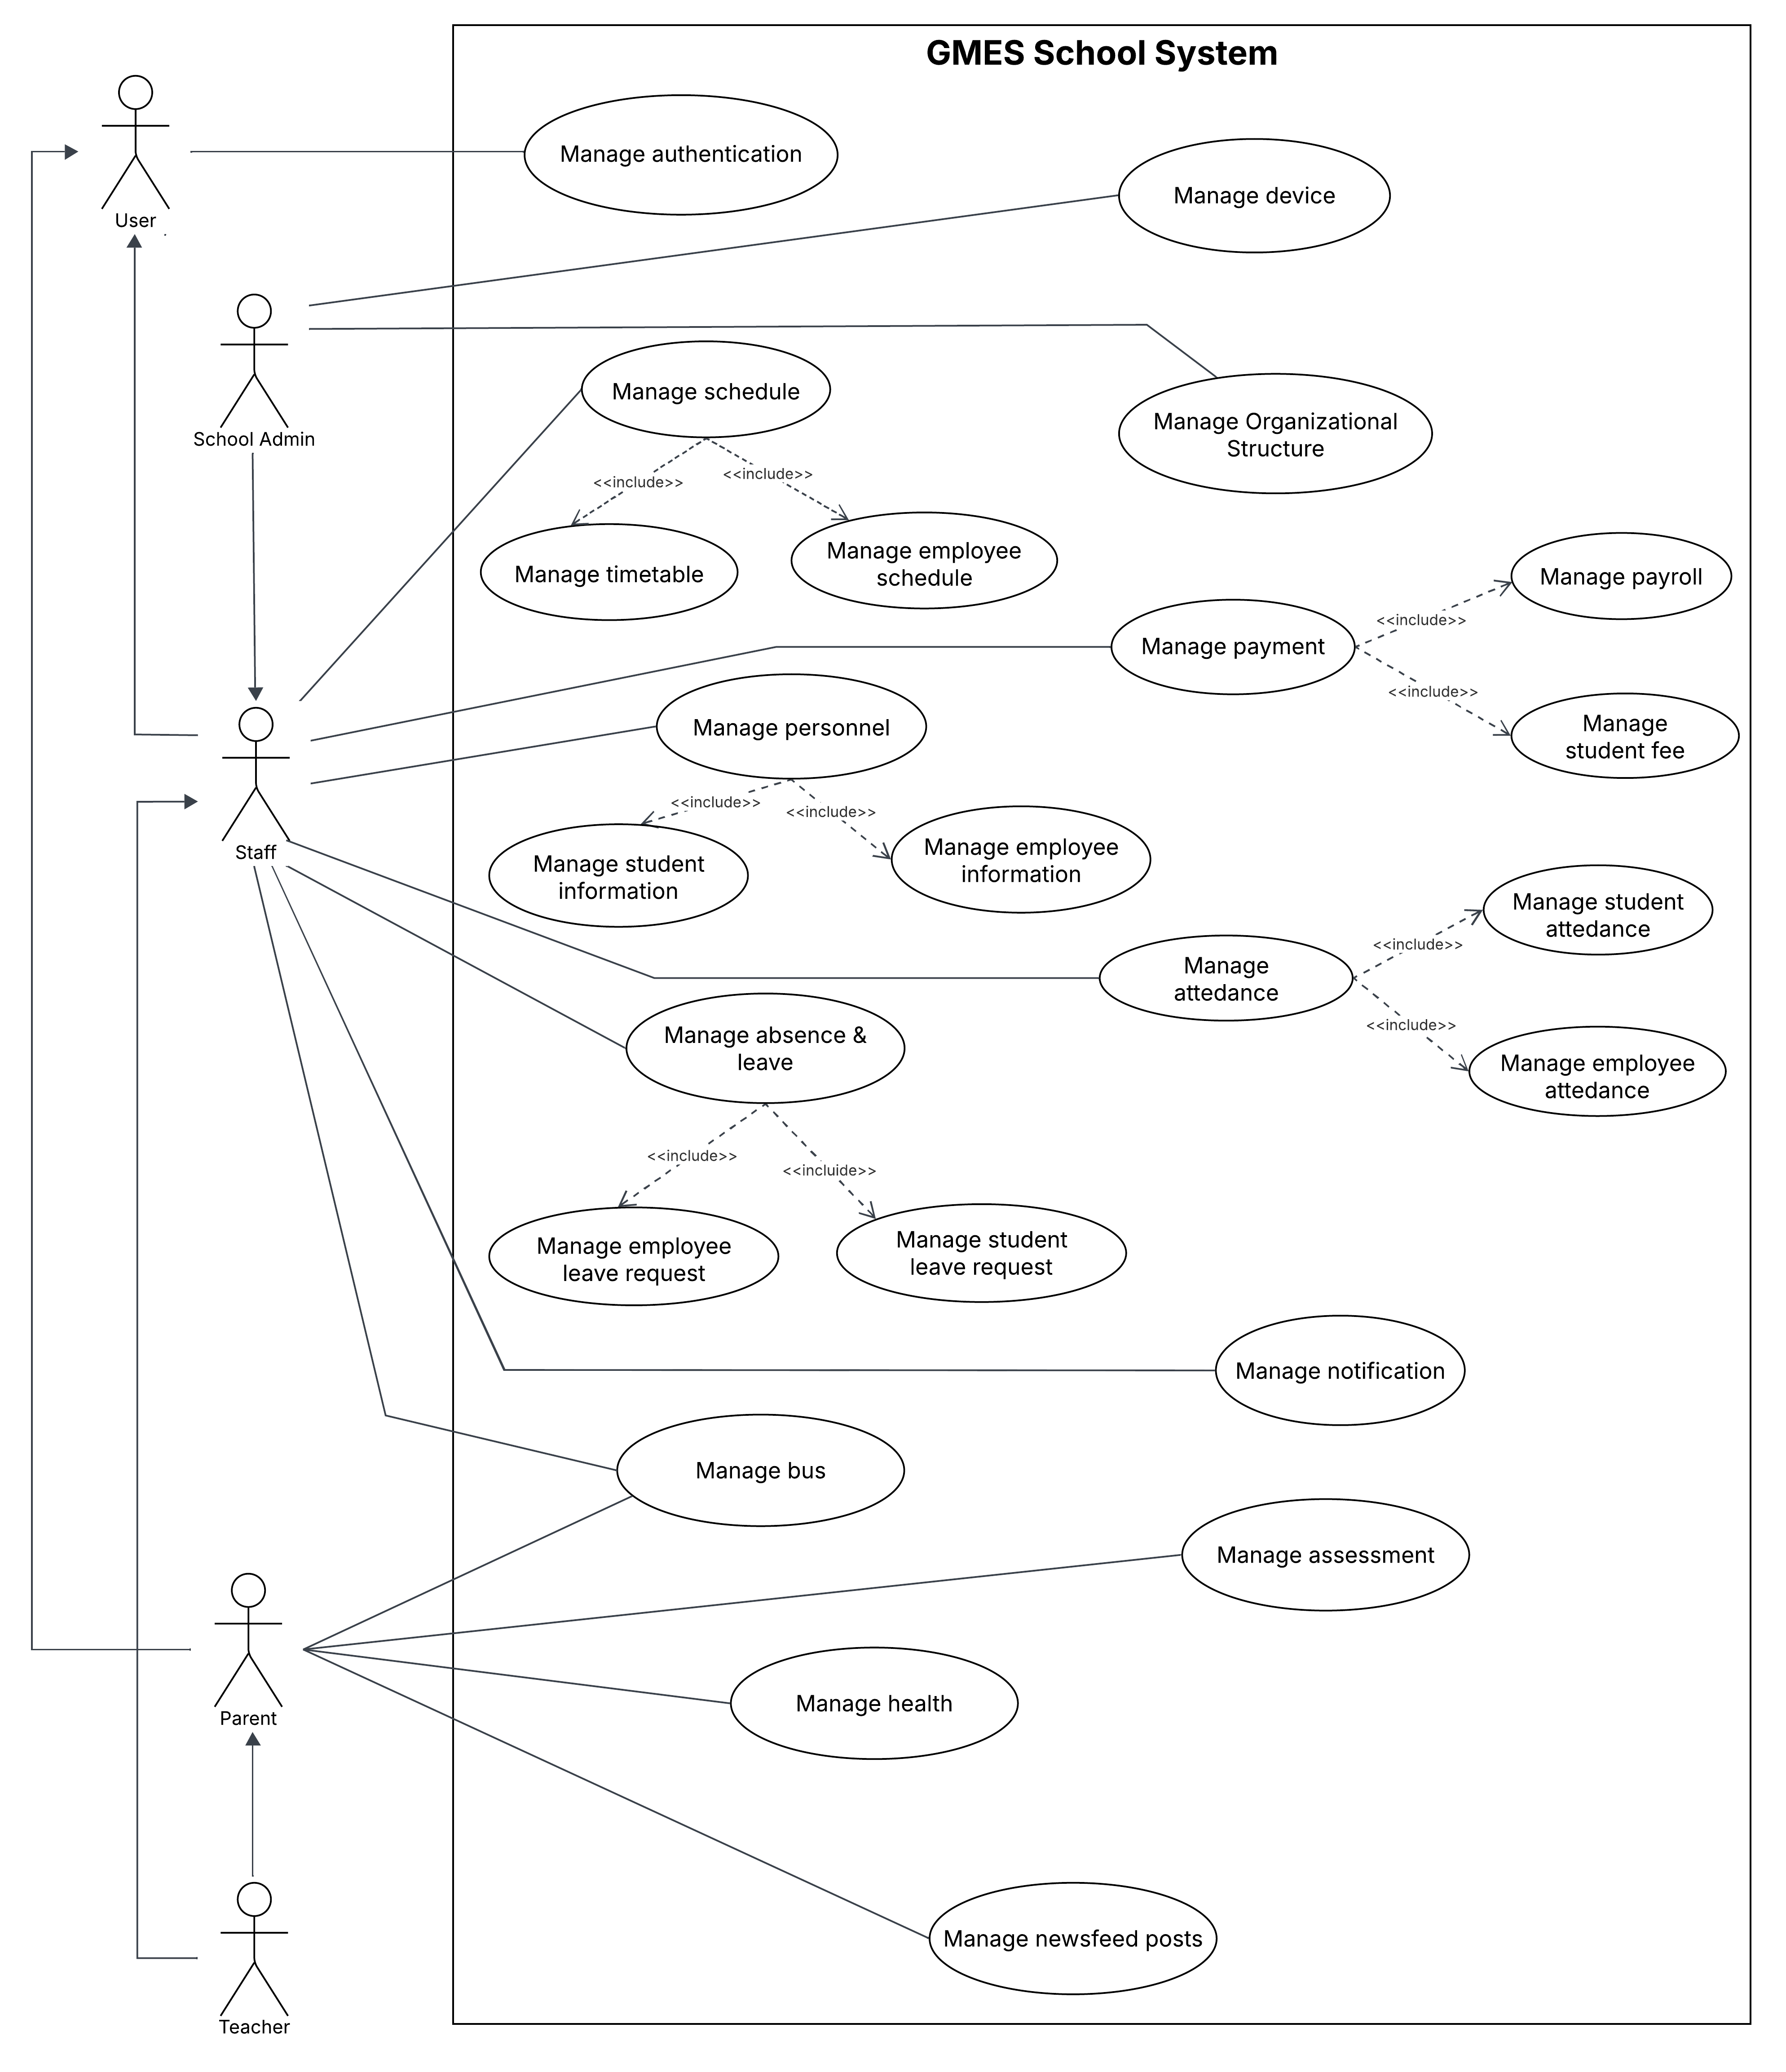
\includegraphics[width=1.1\linewidth]{images/use_case_diagram.png}
    \vspace{-2.5em}
    \caption{System requirements overview.}
    \label{fig:overview_diagram_of_usecases}
\end{figure}

\subsubsection{Detailed System Requirements}
\noindent
\begin{minipage}{\textwidth}
    \setlength{\parindent}{2em}
    This section outlines the detailed system requirements by breaking down each module into specific features. It includes a use case diagram of the \textbf{module assigned to me} and provides an analysis of its key features.
\end{minipage}
\vspace{0.5em}


% ATTENDANCE MANAGEMENT
\newpage
\indent\textbf{2.2.2.1 Attendance Management}
\begin{figure}[H]
    \centering
    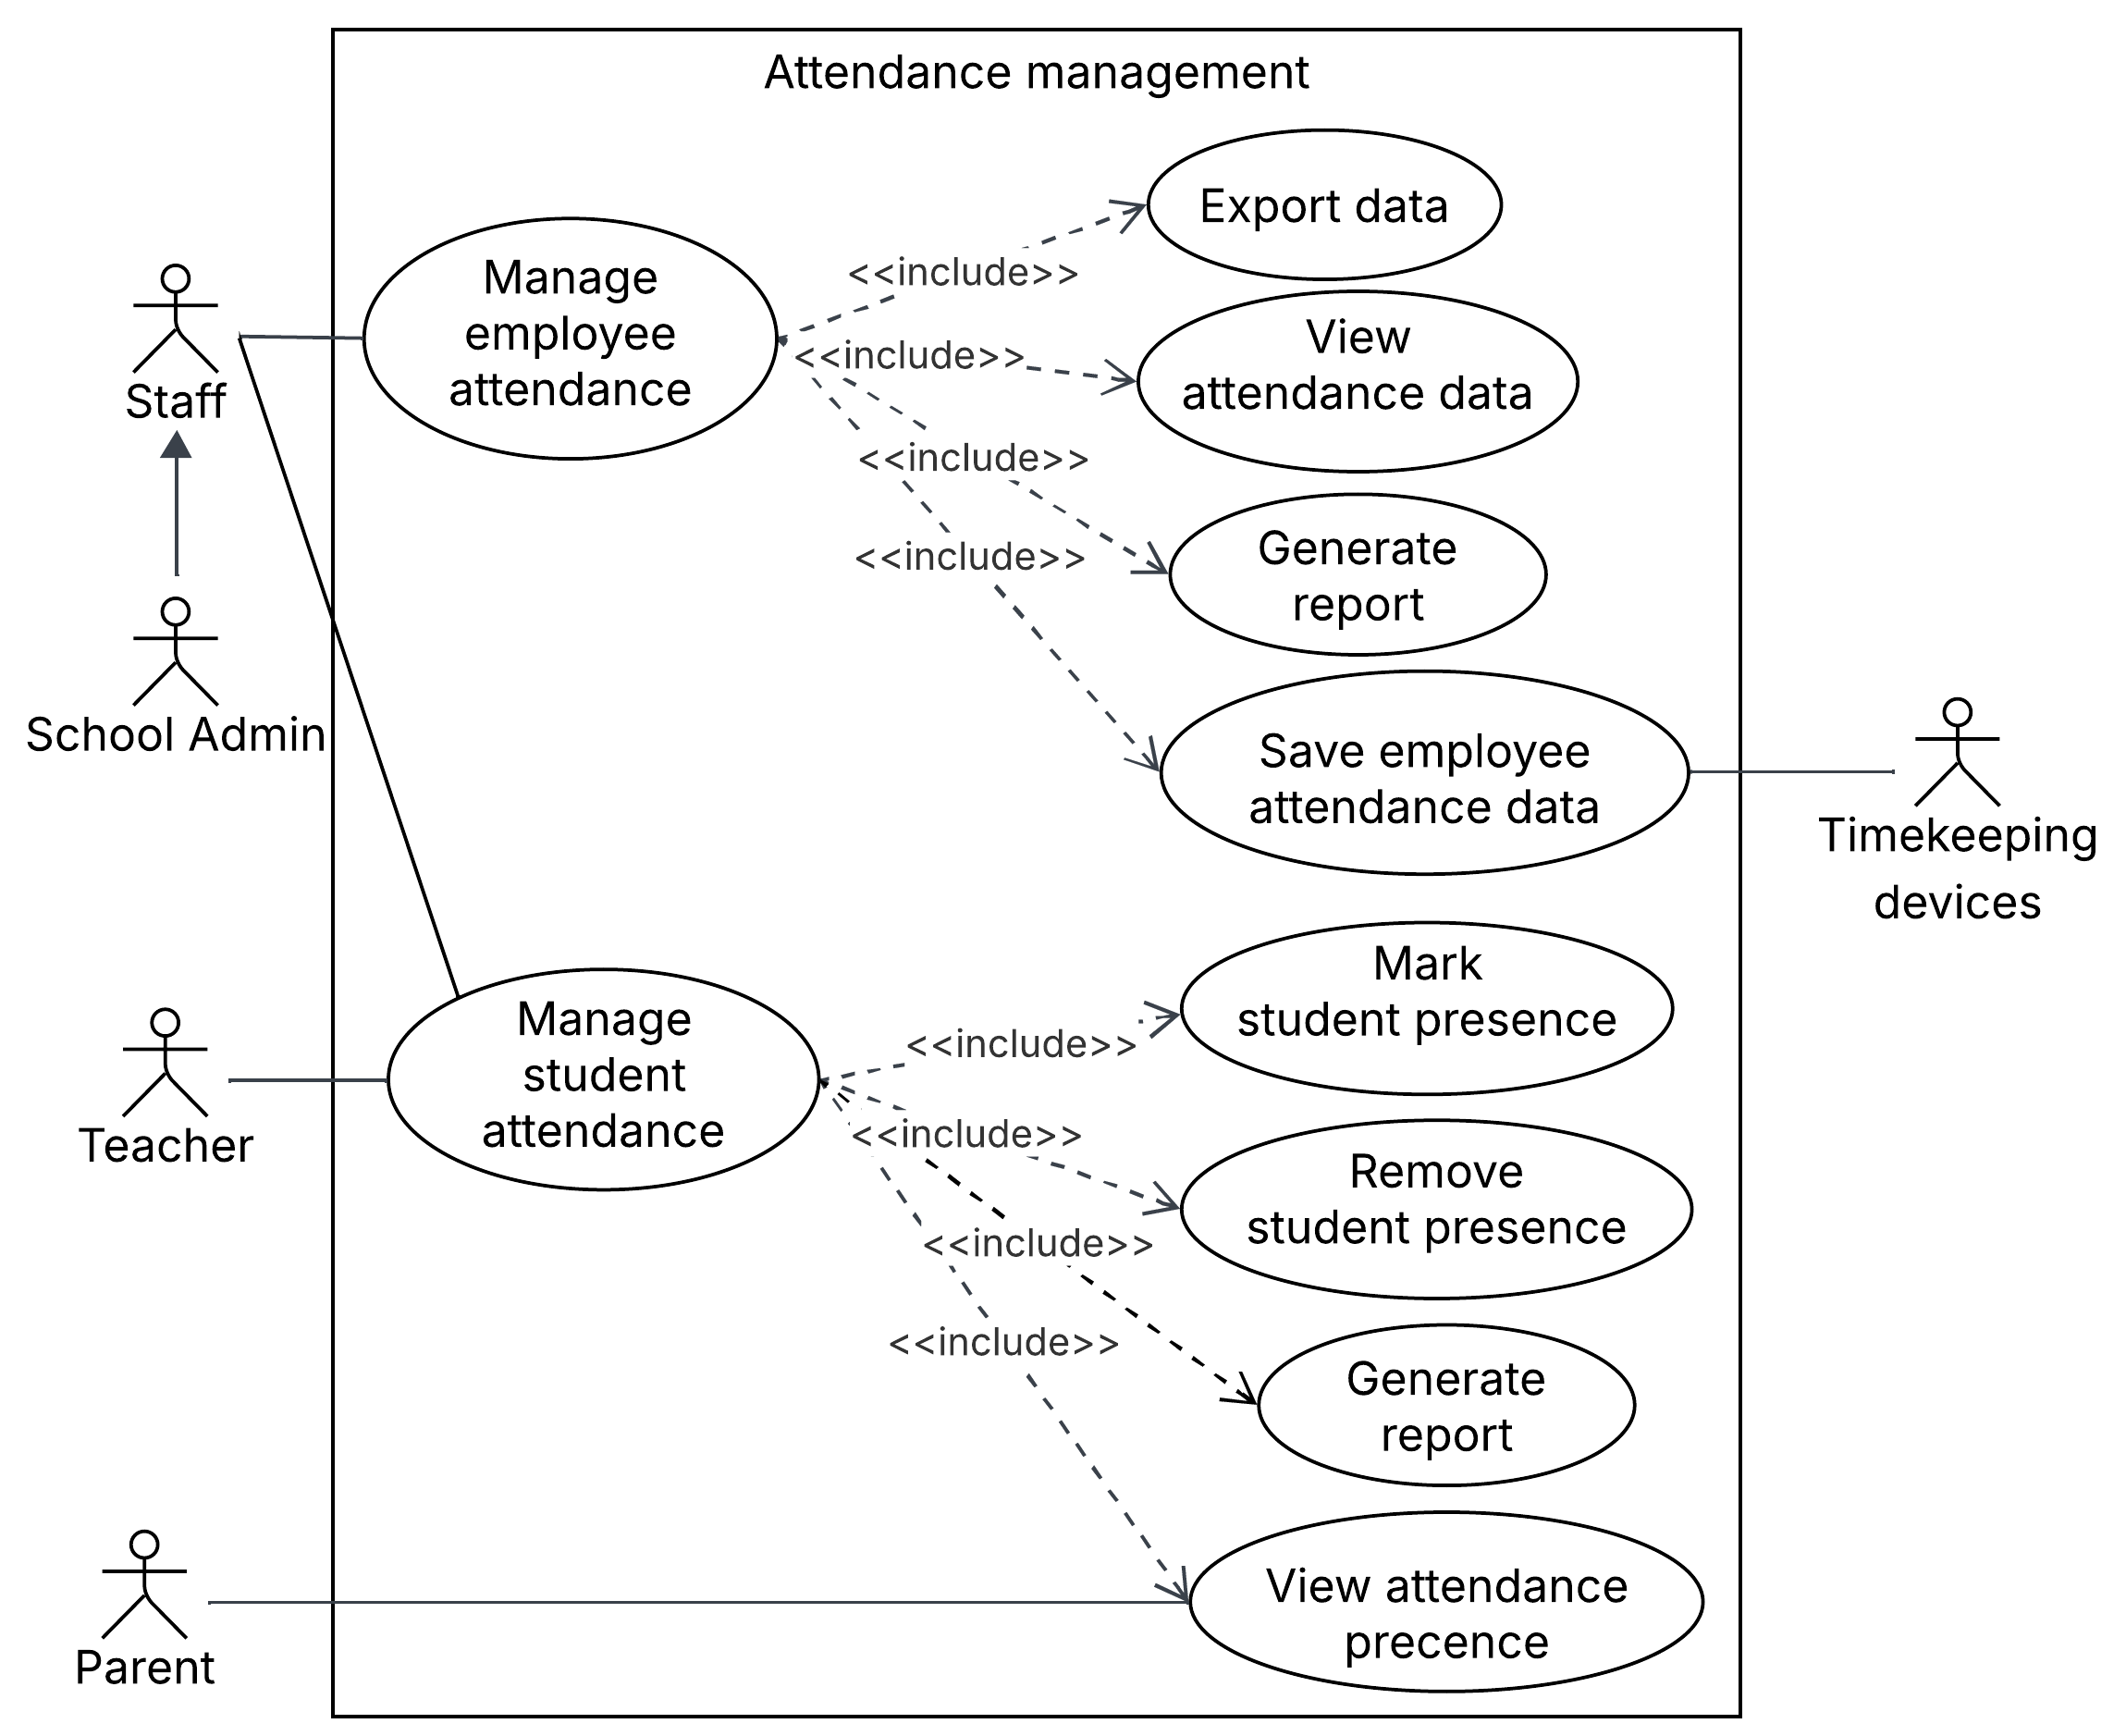
\includegraphics[width=0.7\textwidth]{images/use_case_attendance_management.png}
    \caption{Use case diagram for Attendance Management.}
    \label{fig:use_case_attendance_management}
\end{figure}
In the Attendance Management module, \textbf{the entire sub-module Student Attendance Management has been assigned to me}. The following are its key features:
\begin{itemize}[itemsep=-0.1cm, topsep=0.1cm]
    \item \textbf{Feature 1: Mark students' presence: }is a mobile app feature that enables \textbf{teachers and transportation staff} to efficiently record and update student attendance in class or on the bus with multiple status options. It ensures parents will receive notifications about their child's attendance, providing peace of mind about their safe arrival and participation.
    \item \textbf{Feature 2: Generate report: }is a web app feature that enables \textbf{administrators, authorized staff, and teachers} to create a report and export student/employee attendance data to Excel. This feature replaces manual data collection, minimizing human error, and speeding up processing time.
\end{itemize}

% ASSESSMENT MANAGEMENT
\indent\textbf{2.2.2.2 Student Assessment Management}
\begin{figure}[H]
    \centering
    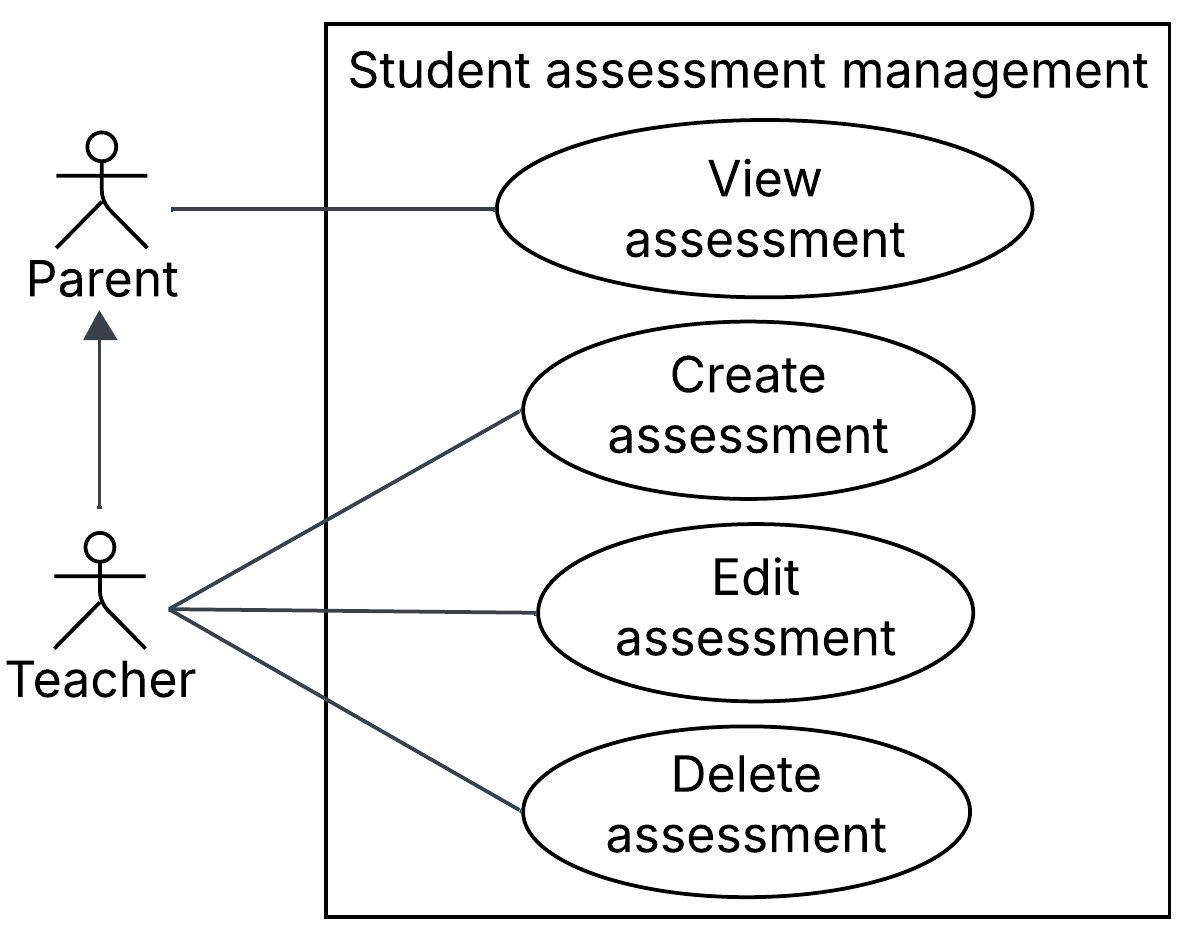
\includegraphics[width=0.4\textwidth]{images/use_case_student_assessment_management.png}
    \caption{Use case diagram for Student Assessment Management.}
    \label{fig:use_case_student_assessment_management}
\end{figure}
The \textbf{entire Student Assessment Management} module for the mobile application \textbf{has been assigned to me}. The following are its key features:
\begin{itemize}[itemsep=-0.1cm, topsep=0.1cm]
    \item \textbf{Feature 1: Create/update assessments:} allows \textbf{teachers} to create or update assessments (with file/image attachments) for their students. This feature eliminates paper-based processes, saves significant preparation time, and enhances quality through multimedia attachments.
    \item \textbf{Feature 2: View assessment:} enables \textbf{parents and teachers} monitor student progress, and performance, allowing them to identify areas where additional support may be needed and collaborate with teachers to develop appropriate solutions.
\end{itemize}

% BUS MANAGEMENT
\indent\textbf{2.2.2.3 Bus Management}
\begin{figure}[H]
    \centering
    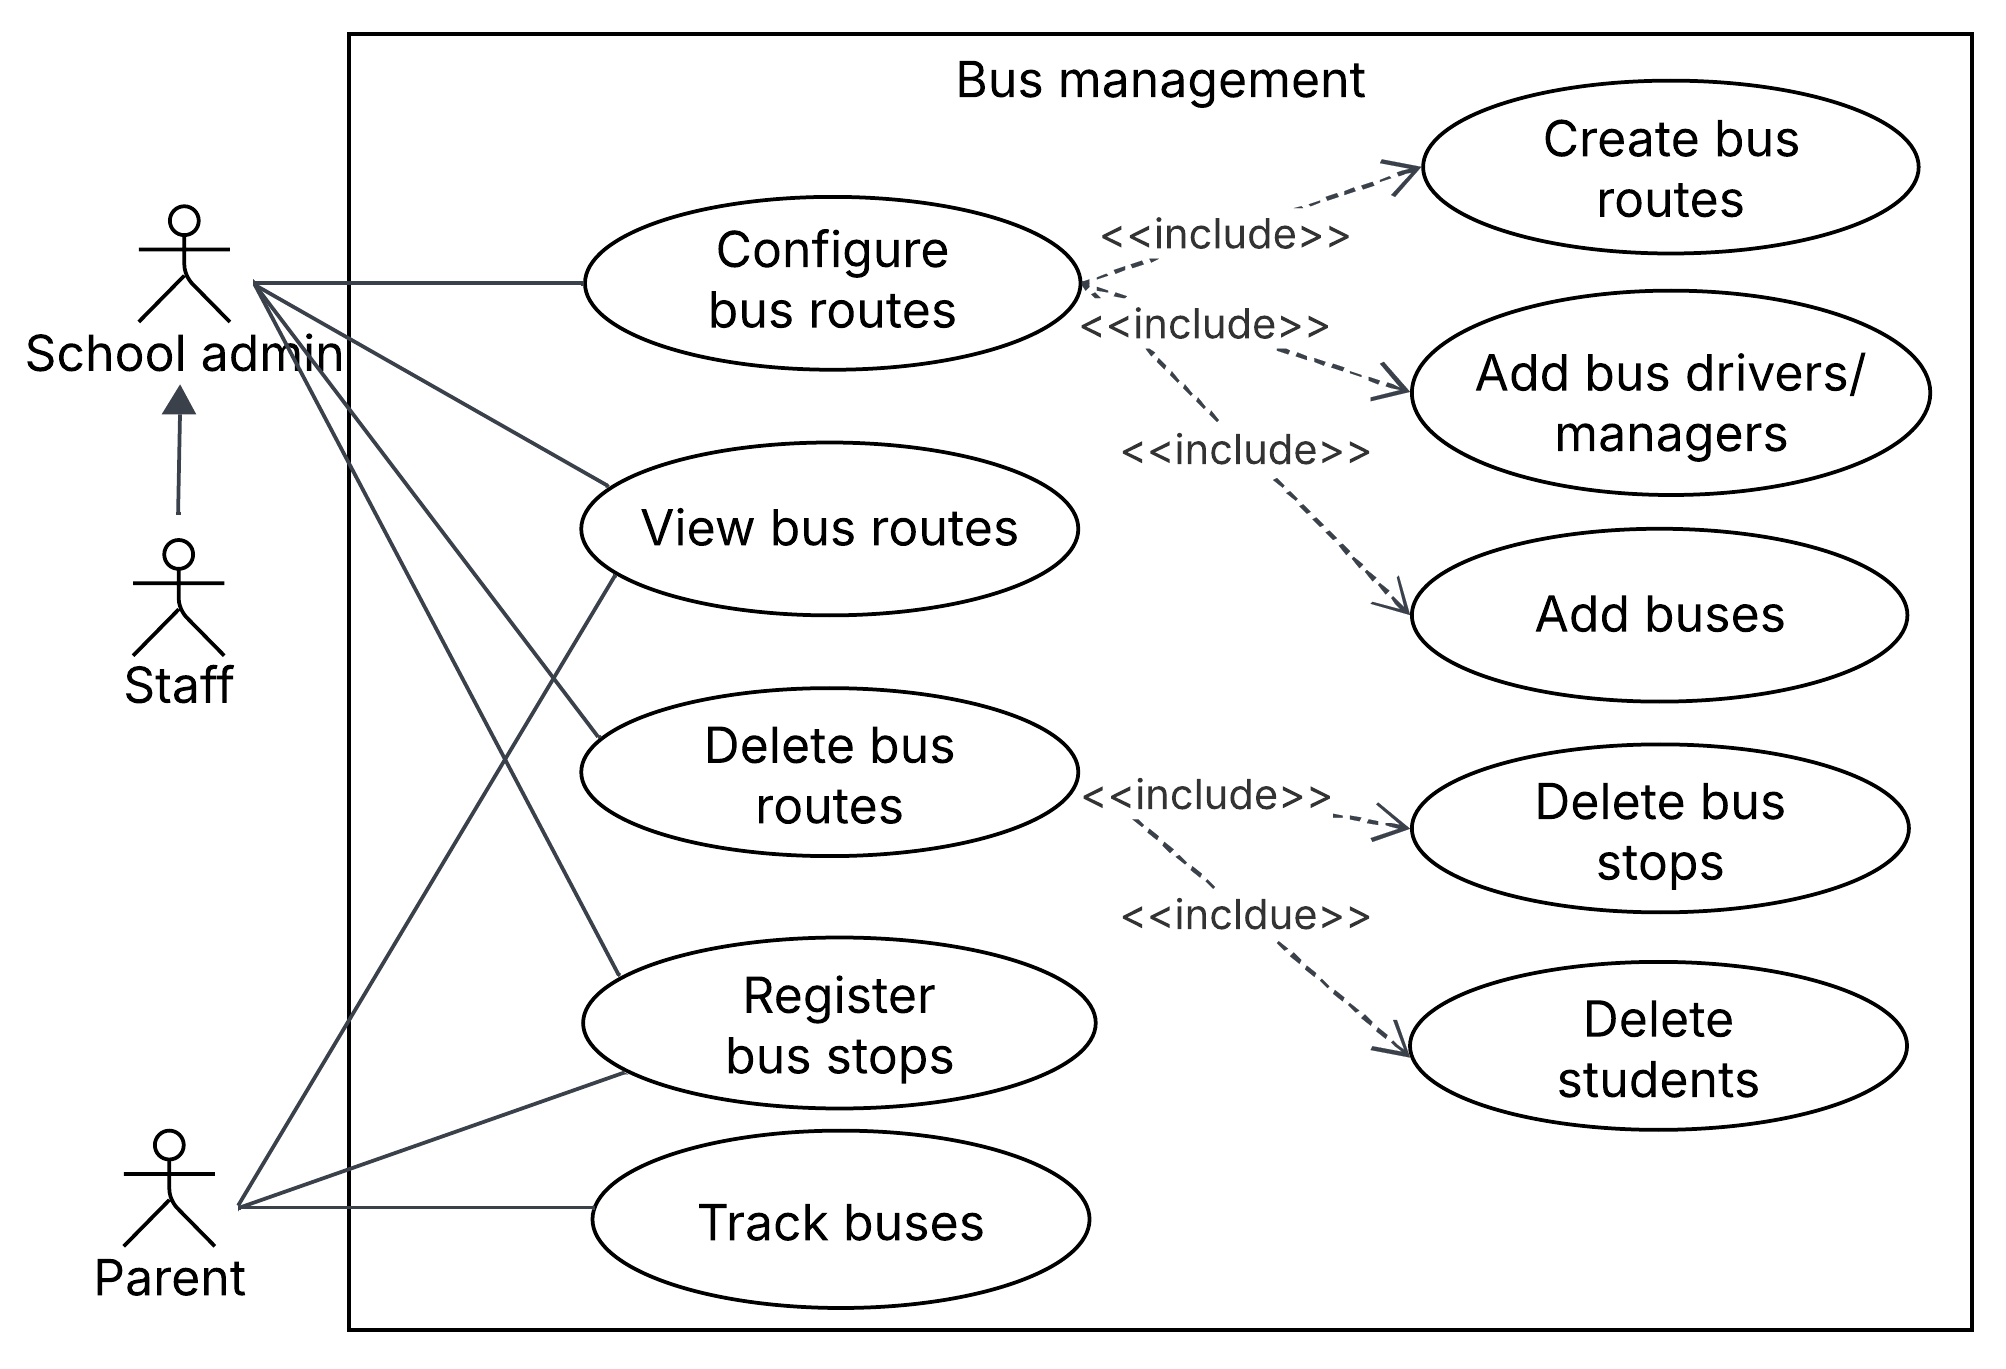
\includegraphics[width=0.7\textwidth]{images/use_case_bus_management.png}
    \caption{Use Case diagram for Bus Management.}
    \label{fig:use_case_bus_management}
\end{figure}
In the Bus Management module, the \textbf{Register Bus Stops} and \textbf{Real-Time Bus Tracking} features for mobile app are \textbf{under my responsibility}. I am also responsible for \textbf{ updating the Configure Bus Route feature} to ensure compatibility with the new Register Bus Stops module. 
\begin{itemize}[itemsep=-0.1cm, topsep=0.1cm]
    \item \textbf{Feature 1: Register bus transportation:} allows \textbf{administrators and parents} to register or cancel bus transportation services for their children. This feature saves time for both parents and staff, reduces paperwork and manual errors.
    \item \textbf{Feature 2: Track buses:} enables \textbf{parents} to monitor their children's school buses in real-time. By displaying the bus's current location, parents can track their child's journey to or from school, ensuring safety and peace of mind. This feature enhances reliability in school transportation services.
\end{itemize}

% HEALTH MANAGEMENT
\indent\textbf{2.2.2.4 Medicine Reminder Management}\\
\indent The \textbf{entire Medicine Reminder Management} module for the mobile application \textbf{has been assigned to me}. The following are its key features:
\begin{itemize}[itemsep=-0.1cm, topsep=0.1cm]
    \item \textbf{Feature 1: Create and update medicine reminder:} allows \textbf{parents} to create or update medicine reminders with image attachments to enhance reliability and clarity of medication information. It ensures that teacher are properly informed about medication schedules and dosage requirements of students.
    \item \textbf{Feature 2: Confirm medicine reminder:} enables \textbf{teachers} to confirm medicine reminder for students.
\end{itemize}
\begin{figure}[H]
    \centering
    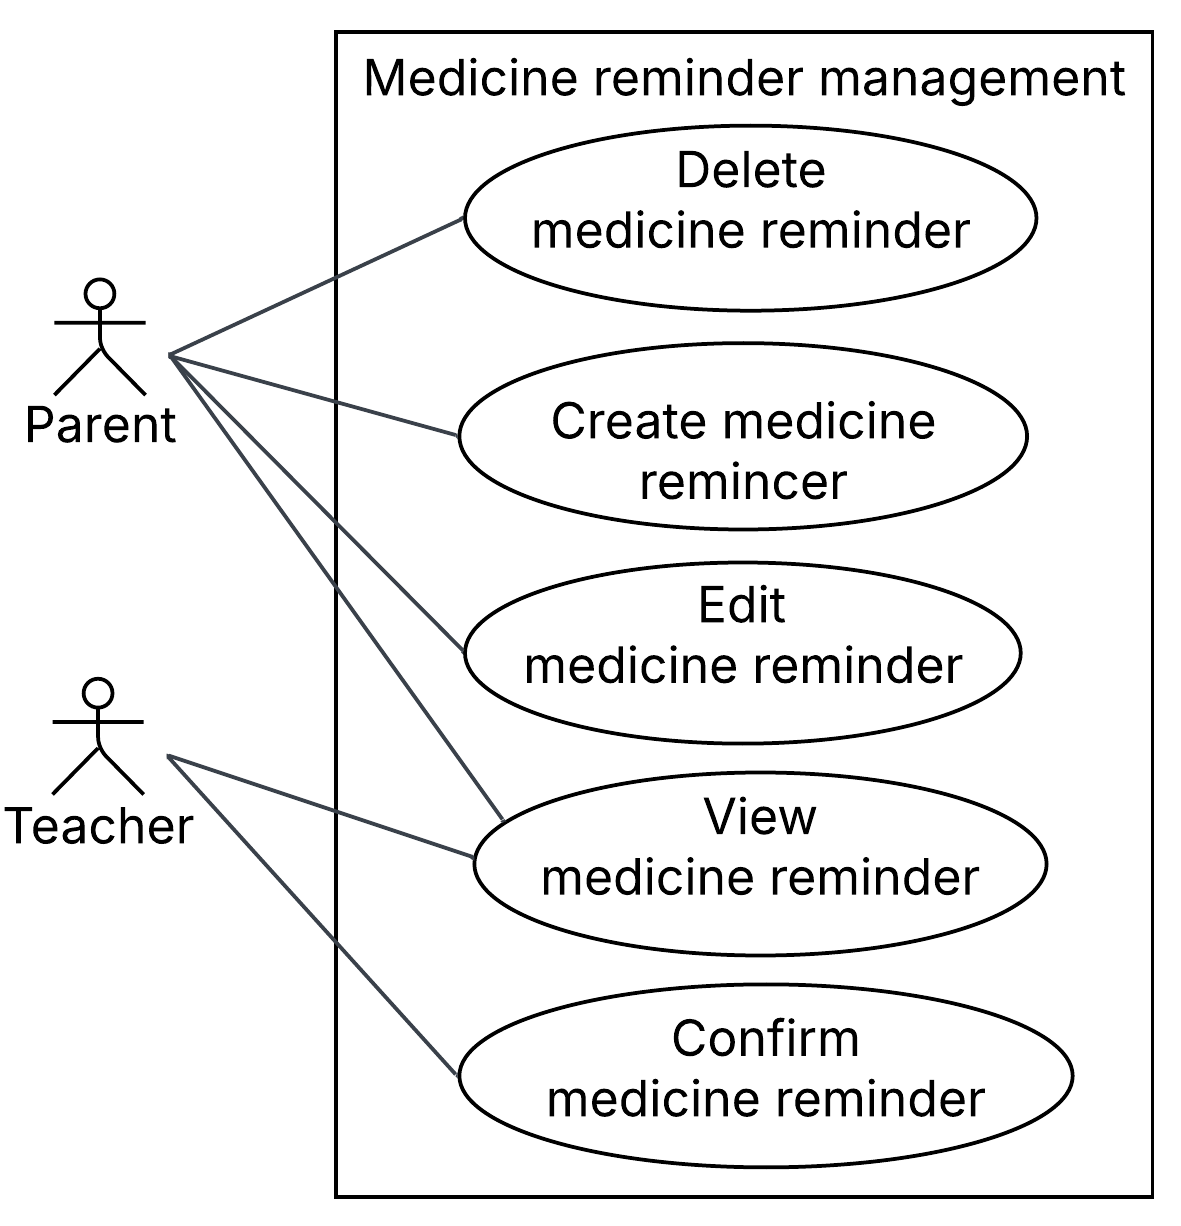
\includegraphics[width=0.45\textwidth]{images/use_case_medicine_reminder.png}
    \caption{Use case diagram for Medicine Reminder Management.}
    \label{fig:use_case_medicine_reminder_management}
\end{figure}

% LEAVE REQUEST MANAGEMENT
\indent\textbf{2.2.2.5 Leave Request Management}
\begin{figure}[H]
    \centering
    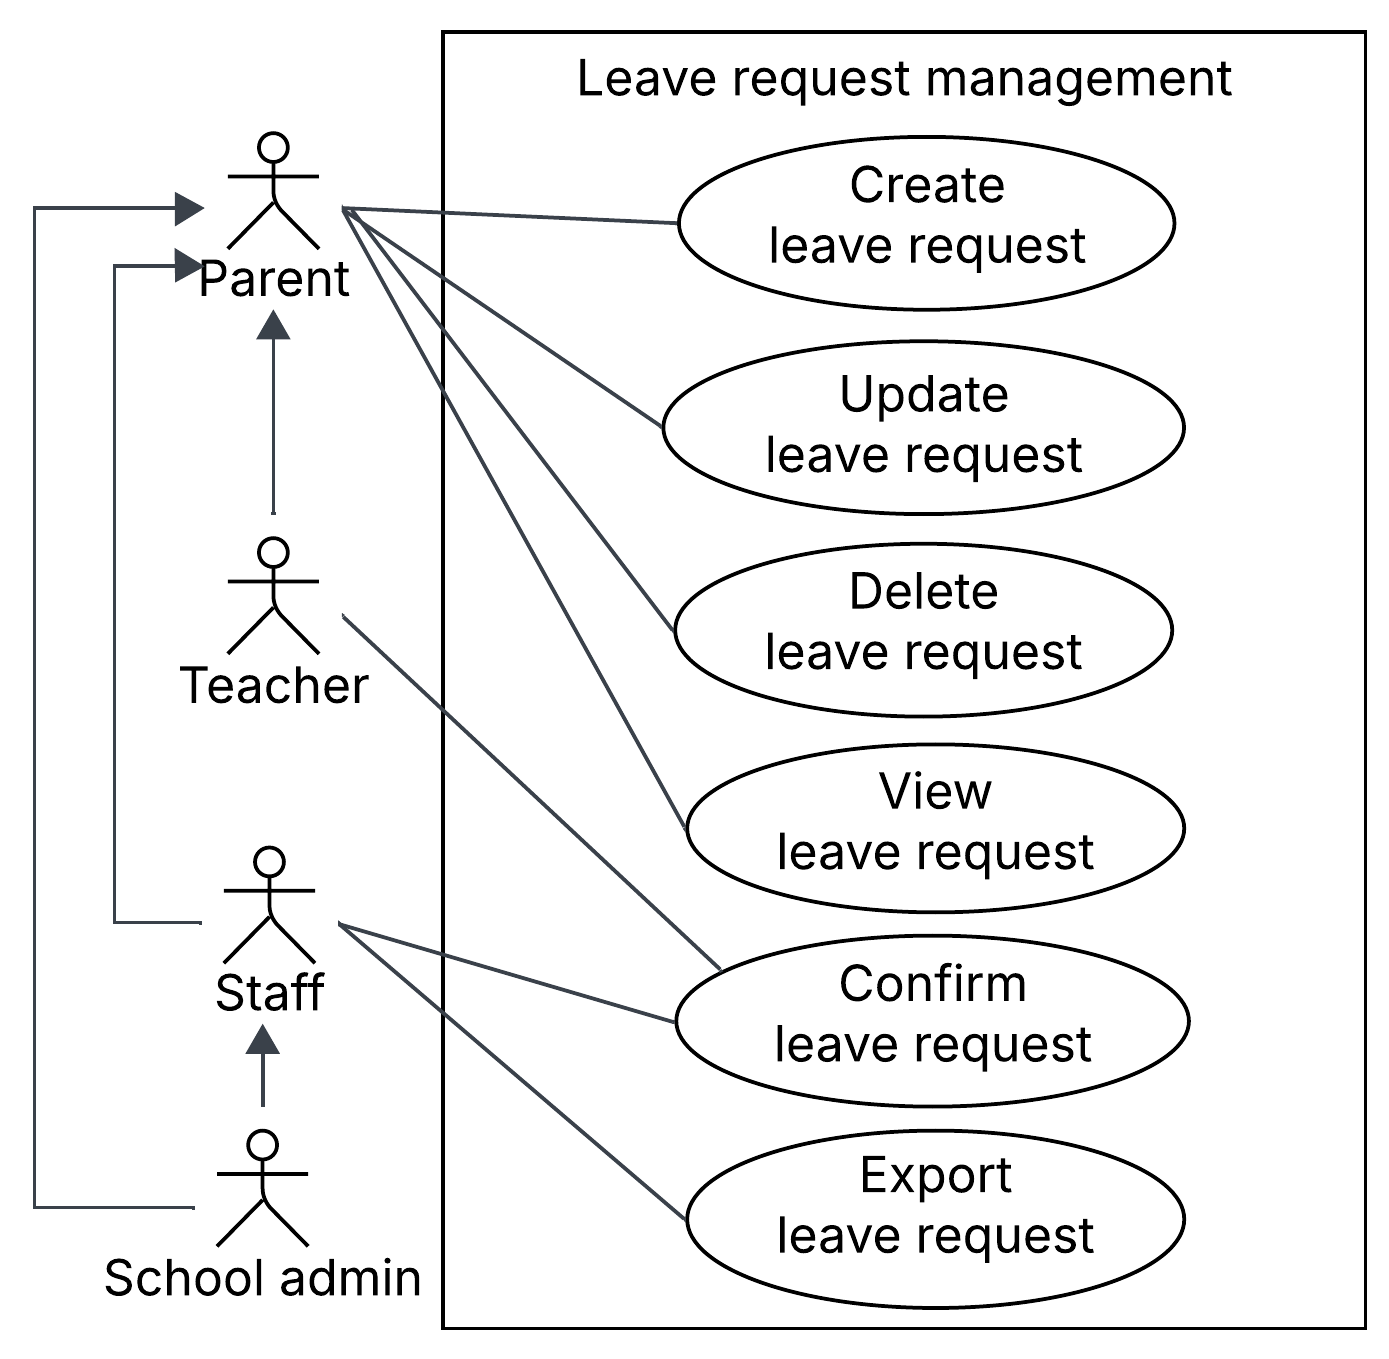
\includegraphics[width=0.5\textwidth]{images/use_case_leave_request_management.png}
    \caption{Use case diagram for Leave Request Management.}
    \label{fig:use_case_leave_request_management}
\end{figure}
Under the Leave Request Management module, the \textbf{entire sub-module Leave Request Management for Mobile App (Parents and Teachers)} is \textbf{assingned to me}. Its \textbf{key features} include the following:
\begin{itemize}[itemsep=-0.1cm, topsep=0.1cm]
    \item \textbf{Feature 1: Create and update leave request: }allows \textbf{parents and teachers} to digitally submit and manage leave requests for themselves or their students. It replaces outdated manual processes and improves transparency and compliance with institutional policies and labor regulations.
    \item \textbf{Feature 2: View and confirm leave request:}
    enables \textbf{teachers} to view their own and students' leave requests, with the ability to approve, decline, or revoke student requests. \textbf{Parents} can only track their child's leave request status.
\end{itemize}

% NEWSFEED MANAGEMENT
\indent\textbf{2.2.2.6 Newsfeed Management}
\begin{figure}[H]
    \centering
    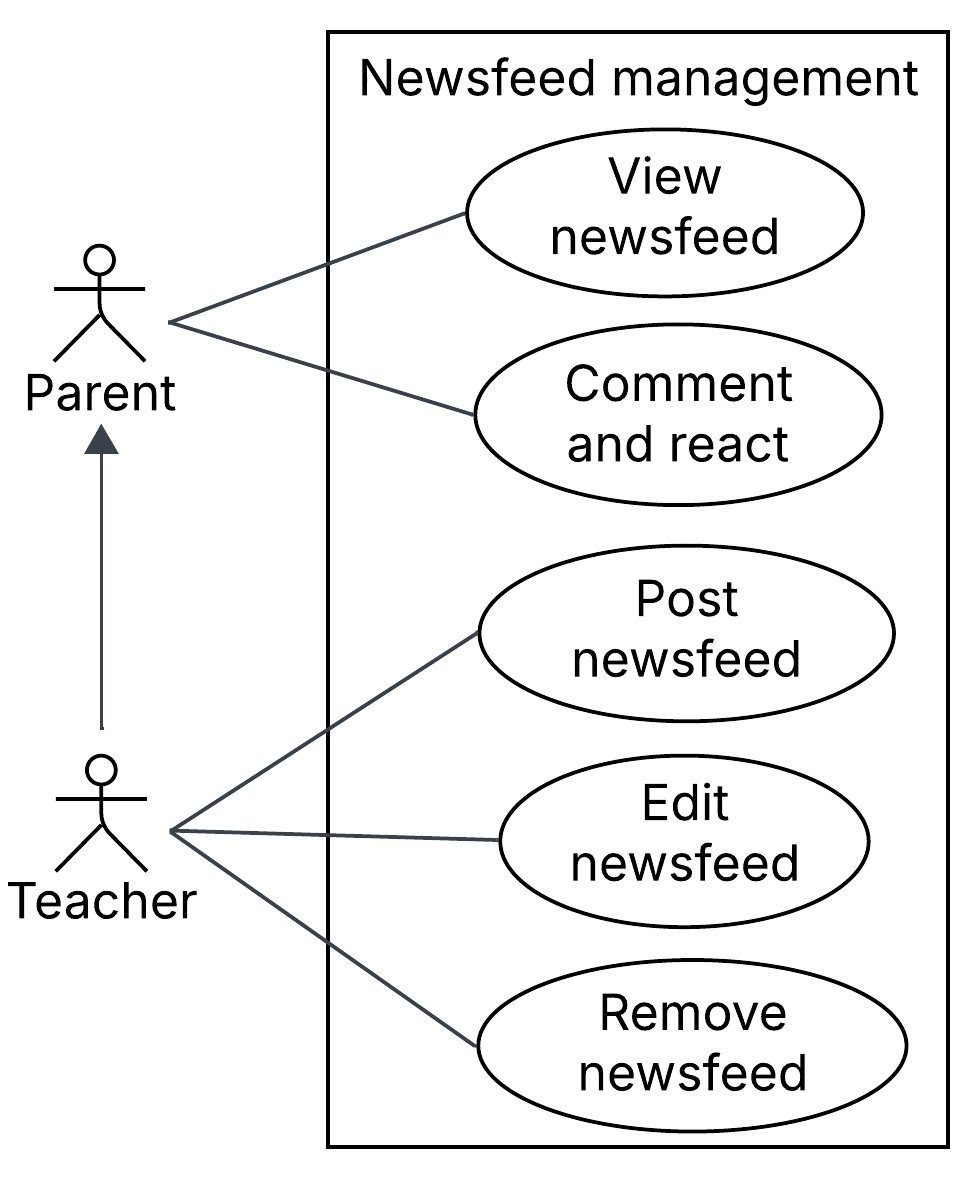
\includegraphics[width=0.35\textwidth]{images/use_case_newsfeed_management.png}
    \vspace{-0.5em}
    \caption{Use case diagram for Newsfeed Management.}
    \label{fig:use_case_newsfeed_management}
\end{figure}
The \textbf{entire Newsfeed Management module is assigned to me}. The module's \textbf{key features} include:
\begin{itemize}[itemsep=-0.1cm, topsep=0.1cm]
    \item \textbf{Feature 1: Create/update newsfeeds:} allows \textbf{teachers} to create or update posts (with file/image/video attachments) to share class events and activities with parents. This feature significantly improves communication between schools and families and ensures parents stay actively involved in their children's school life.
    \item \textbf{Feature 2: View and interact with post:} enables \textbf{parents and teachers} to view, comment on, and react to posts.
\end{itemize}

% NOTIFICATION MANAGEMENT
\indent\textbf{2.2.2.7 Notification Management}
\begin{figure}[H]
    \centering
    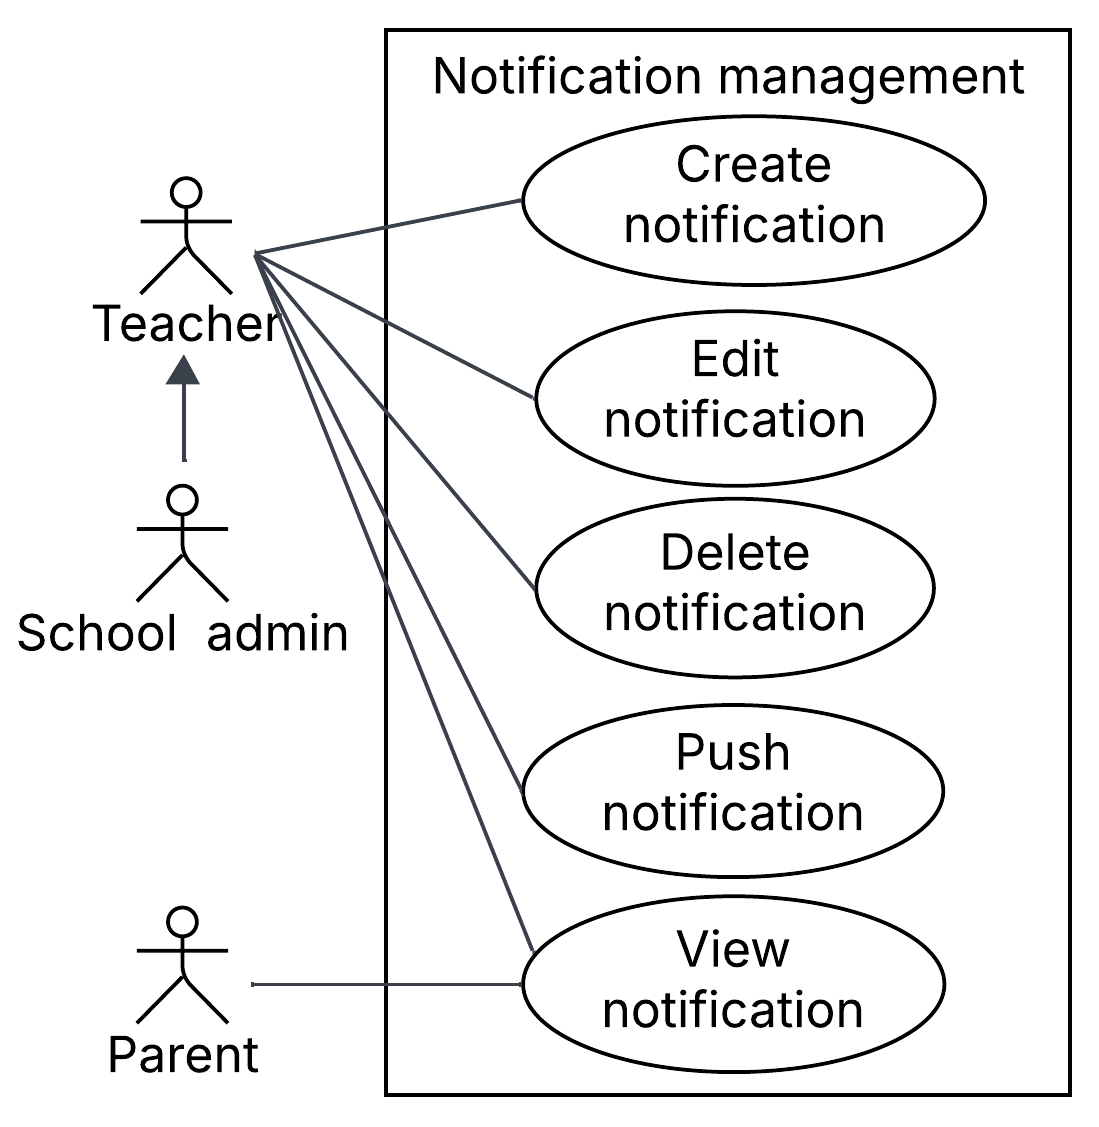
\includegraphics[width=0.4\textwidth]{images/use_case_notification_management.png}
    \caption{Use Case diagram for Notification Management.}
    \label{fig:use_case_notification_management}
\end{figure}
The \textbf{entire Notification Management module is assigned to me}. The module's \textbf{key features} include:
\begin{itemize}[itemsep=-0.1cm, topsep=0.1cm]
    \item \textbf{Feature 1: Create and push notification:} allows \textbf{administrators, authorized staff, and teachers} to create and push notifications to employees and parents through email and mobile notification channels. This feature ensures employees and parents are informed about critical notifications, events, and important updates.
\end{itemize}

% PERSONNEL MANAGEMENT
\indent\textbf{2.2.2.8 Personnel management}
\begin{figure}[H]
    \centering
    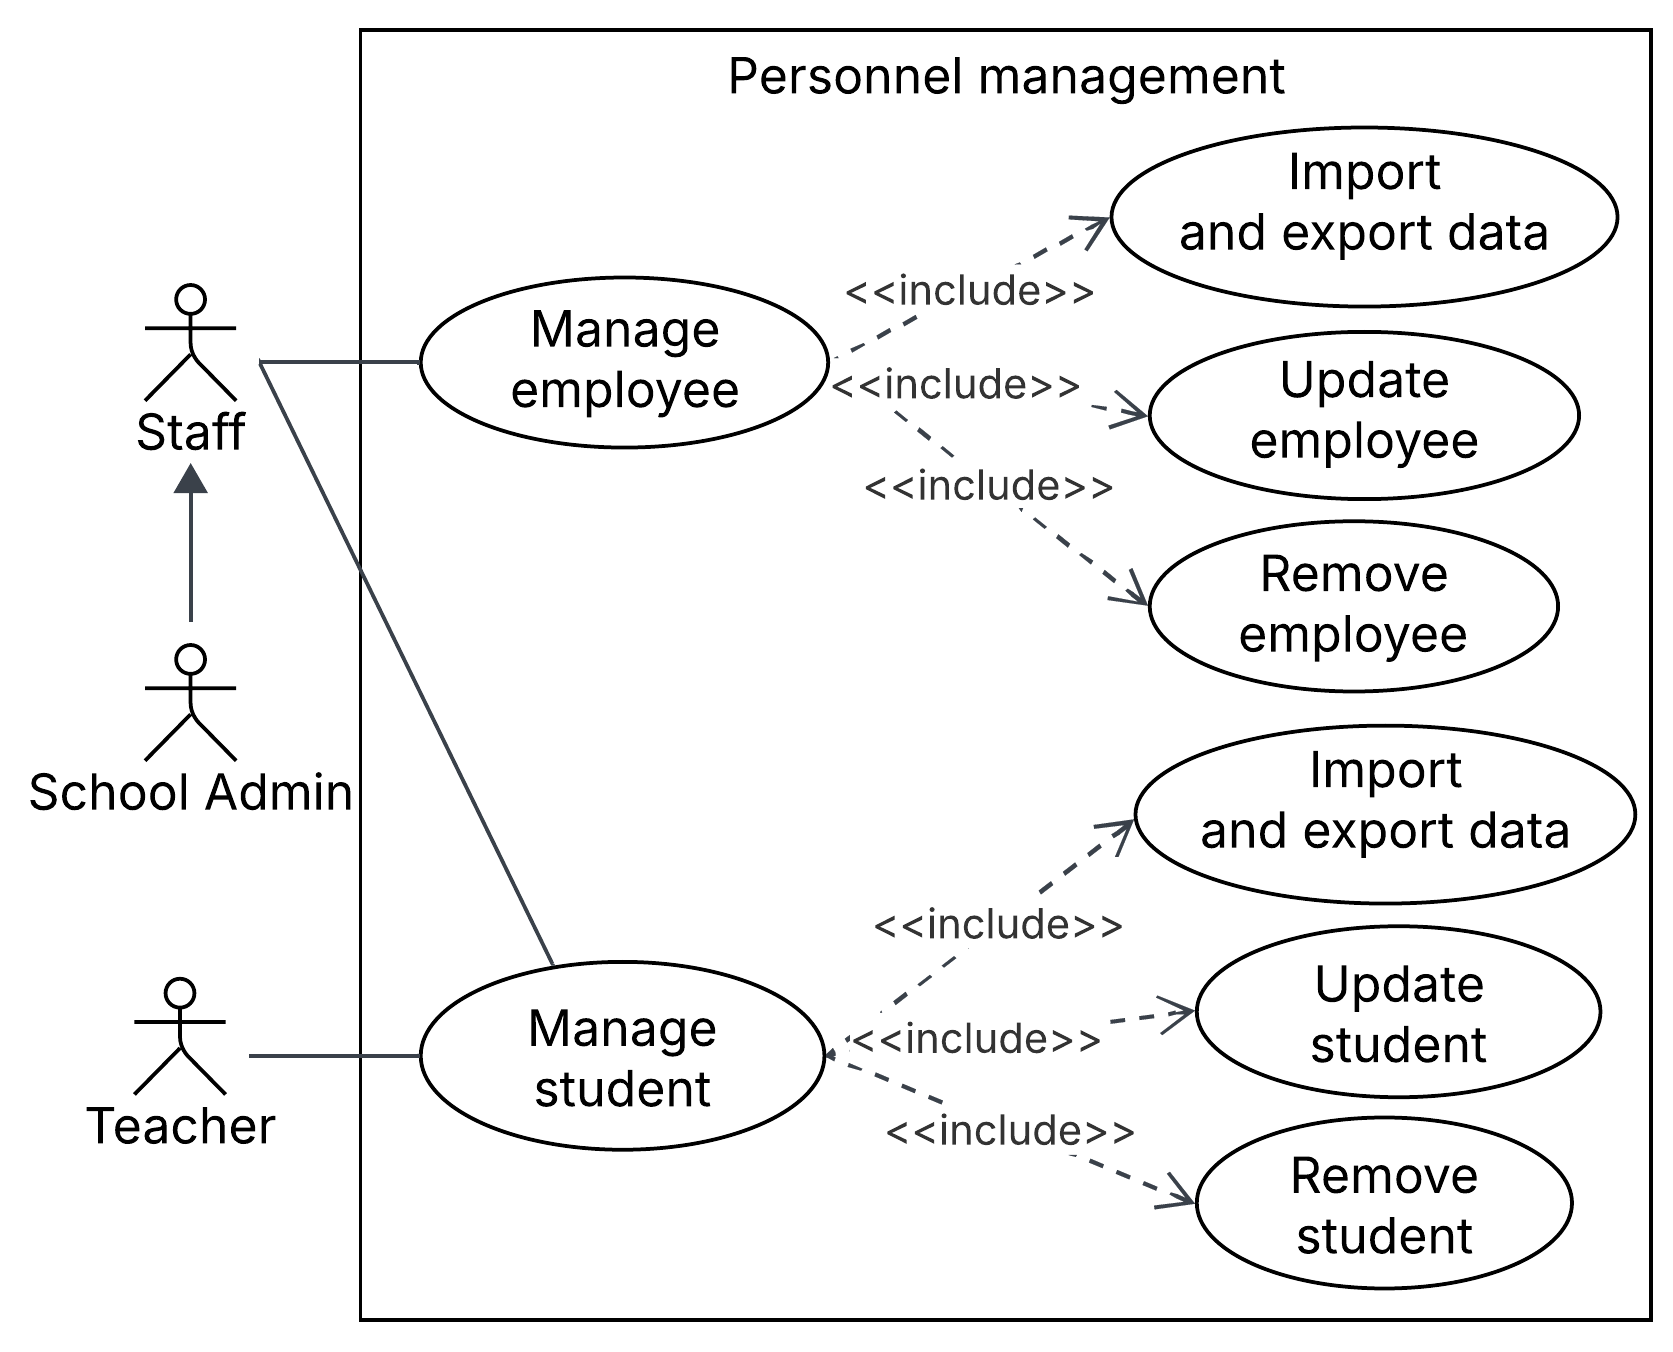
\includegraphics[width=0.6\textwidth]{images/use_case_personnel_management.png}
    \caption{Use case diagram for Personnel Management.}
    \label{fig:use_case_personnel_management}
\end{figure}
Under the the Personnel Management module, my responsibilities include developing the \textbf{Import/Export} functionality for employee and student data.
\begin{itemize}[itemsep=-0.1cm, topsep=0.1cm]
    \item \textbf{Feature 1: Import employee/student data: }allows \textbf{administrators and authorized staff} to efficiently create and update multiple employee/student data into the system, via Excel or ERP. This feature significantly reduces time, and effort and minimizes errors.
    \item \textbf{Feature 2: Export employee/student data: }allows \textbf{administrators and authorized staff} to export employee/student data to Excel for reporting purposes.
\end{itemize}